\newpage
\section{迁移学习的研究领域} %--------c----------------------

依据目前较流行的机器学习分类方法,机器学习主要可以分为有监督、半监督和无监督机器学习三大类。同理,迁移学习也可以进行这样的分类。需要注意的是,依据的分类准则不同,分类结果也不同。在这一点上,并没有一个统一的说法。我们在这里仅根据目前较流行的方法,对迁移学习的研究领域进行一个大致的划分。

图~\ref{fig-area}给出了迁移学习的常用分类方法总结。

\begin{figure}[htbp]
	\centering
	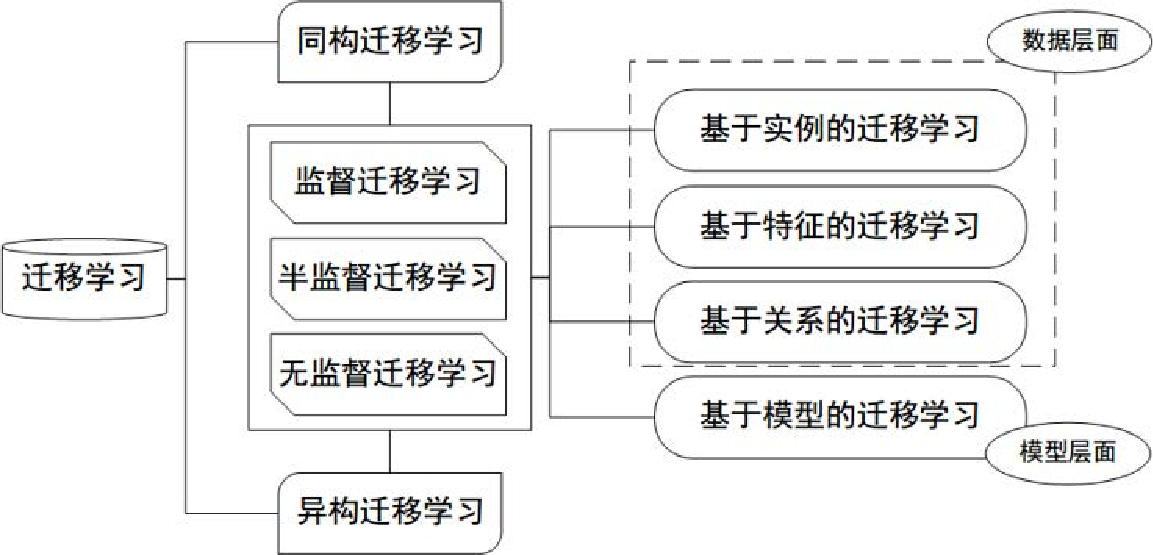
\includegraphics[scale=0.6]{./figures/fig-area.pdf}
	\caption{迁移学习的研究领域与研究方法分类}
	\label{fig-area}
\end{figure}

大体上讲,迁移学习的分类可以按照四个准则进行:\textit{按目标域有无标签分、按学习方法分、按特征分、按离线与在线形式分}。不同的分类方式对应着不同的专业名词。当然,即使是一个分类下的研究领域,也可能同时处于另一个分类下。下面我们对这些分类方法及相应的领域作简单描述。

\subsection{按目标域标签分}
这种分类方式最为直观。类比机器学习,按照目标领域有无标签,迁移学习可以分为以下三个大类:

\begin{enumerate}
	\item 监督迁移学习 (Supervised Transfer Learning)
	\item 半监督迁移学习 (Semi-Supervised Transfer Learning)
	\item 无监督迁移学习 (Unsupervised Transfer Learning)
\end{enumerate}

显然,少标签或无标签的问题(半监督和无监督迁移学习),是研究的热点和难点。这也是本手册重点关注的领域。

\subsection{按学习方法分类}
按学习方法的分类形式,最早在迁移学习领域的权威综述文章~\cite{pan2010survey}给出定义。它将迁移学习方法分为以下四个大类:

\begin{enumerate}
	\item 基于样本的迁移学习方法 (Instance based Transfer Learning)
	\item 基于特征的迁移学习方法 (Feature based Transfer Learning)
	\item 基于模型的迁移学习方法 (Model based Transfer Learning)
	\item 基于关系的迁移学习方法 (Relation based Transfer Learning)
\end{enumerate}

这是一个很直观的分类方式,按照数据、特征、模型的机器学习逻辑进行区分,再加上不属于这三者中的关系模式。

基于实例的迁移,简单来说就是通过权重重用,对源域和目标域的样例进行迁移。就是说直接对不同的样本赋予不同权重,比如说相似的样本,我就给它高权重,这样我就完成了迁移,非常简单非常非常直接。

基于特征的迁移,就是更进一步对特征进行变换。意思是说,假设源域和目标域的特征原来不在一个空间,或者说它们在原来那个空间上不相似,那我们就想办法把它们变换到一个空间里面,那这些特征不就相似了?这个思路也非常直接。这个方法是用得非常多的,一直在研究,目前是感觉是研究最热的。

基于模型的迁移,就是说构建参数共享的模型。这个主要就是在神经网络里面用的特别多,因为神经网络的结构可以直接进行迁移。比如说神经网络最经典的finetune就是模型参数迁移的很好的体现。

基于关系的迁移,这个方法用的比较少,这个主要就是说挖掘和利用关系进行类比迁移。比如老师上课、学生听课就可以类比为公司开会的场景。这个就是一种关系的迁移。

目前最热的就是基于特征还有模型的迁移,然后基于实例的迁移方法和他们结合起来使用。

迁移学习方法是本手册的重点。我们在后续的篇幅中介绍。

\subsection{按特征分类}

按照特征的属性进行分类,也是一种常用的分类方法。这在最近的迁移学习综述~\cite{weiss2016survey}中给出。按照特征属性,迁移学习可以分为两个大类:

\begin{enumerate}
	\item 同构迁移学习 (Homogeneous Transfer Learning)
	\item 异构迁移学习 (Heterogeneous Transfer Learning)
\end{enumerate}

这也是一种很直观的方式:如果特征语义和维度都相同,那么就是同构;反之,如果特征完全不相同,那么就是异构。举个例子来说,不同图片的迁移,就可以认为是同构;而图片到文本的迁移,则是异构的。

\subsection{按离线与在线形式分}

按照离线学习与在线学习的方式,迁移学习还可以被分为:

\begin{enumerate}
	\item 离线迁移学习 (Offline Transfer Learning)
	\item 在线迁移学习 (Online Transfer Learning)
\end{enumerate}

目前,绝大多数的迁移学习方法,都采用了离线方式。即,源域和目标域均是给定的,迁移一次即可。这种方式的缺点是显而易见的:算法无法对新加入的数据进行学习,模型也无法得到更新。与之相对的,是在线的方式。即随着数据的动态加入,迁移学习算法也可以不断地更新。